\chapter{Вступ}
\section{Теоретичні відомості до першого завдання}
\subsection{Алгебра логіки}
\textbf{Алгебра логіки} \emph{(Булева логіка, двійкова логіка, двійкова алгебра)} — розділ математичної логіки, що вивчає систему логічних операцій над висловлюваннями. Вважається, що висловлювання можуть бути тільки істинними або помилковими, тобто використовується так звана \emph{бінарна або двійкова логіка}.

Булева функція задається у вигляді таблиці, або графіка зі стандартним (лексикографічним) розташуванням наборів аргументів,виконана кодом Грея.

\textbf{Код Грея} — одна із систем кодування інформації, в якій два послідовні коди відрізняються значенням лише одного біта.

\textbf{Табли́ця істинності} — математична таблиця, що широко використовується у математичній логіці зокрема в алгебрі логіки, численні висловлень для обчислення значень булевих функцій.

Приклад таблиці істинності:
\begin{center}
\begin{table}[h!]
\begin{tabu}{ | X[-3,l] | X[-3,l] | X[-3,l] | X[-3,l] |}
\hline
N &$X_{1}$ & $X_{2}$ & $F_{1}$ \\
 \hline
0 & 0 & 0 & 0  \\
\hline
1 &  0 & 1  &  0  \\
\hline
2 & 1 & 0 & 0   \\
\hline
3 & 1 & 1 & 1  \\
\hline
\end{tabu}
\vspace{6mm}\\
\caption{Приклад таблиці істинності}\label{tab:logic_truth_table_ex}
\end{table}
\end{center}
\newpage
\subsection{Базові логічні вирази}
Відомі такі основні логічні вирази, як:
\begin{itemize}
	\item Інверсія (логічне  'НЕ', NOT,$\lnot$)
	\item Кон'юнкція (логічне множення, логічне  І, AND,$\wedge$)
	\item Диз'юнкція (логічне додавання, логічне  АБО, OR,$\lor$)
	\item Виключне АБО(Сума по модулю 2,XOR,$\oplus$)
\end{itemize}

Також існують логічні вирази для базисів(детально розглядаються на сторінці  \pageref{subsect:logic_basis}).
\newpage
\subsection{Форма подання логічних виразів}
Логічний вираз який є тотожний функції можна подати у трьох загальних виглядах:
\begin{itemize}
	\item Диз'юнктивна нормальна форма (ДНФ)
	\item Кон'юнктивна нормальна форма (КНФ)
	\item Алгебраїчна нормальна форма (АНФ або поліном Жегалкіна)
\end{itemize}
\newpage
\subsection{Дії над логічними виразами}
Для логічних виразів існують такі закони алгебри:
\begin{center}
\begin{table}[h!]
\begin{tabu} { | X[3,с] | X[3,c] | X[3,c] | }
 \hline
Назва закону& АБО & І \\
 \hline
 Переміщення &$A \lor B = B \lor A$  &$A \wedge B = B \wedge A $  \\
\hline
 Комбінування &$A \lor (B \lor C)= (A \lor B) \lor C $  &$A \wedge (B \wedge C)= (A \wedge B) \wedge C $  \\
\hline
Розподільний &$(A \lor B) \wedge C= A \wedge C \lor B \wedge C $  \vspace{1mm}&$(A \wedge B) \lor C= A \lor C \wedge B \lor C $ \vspace{1mm}   \\
\hline
Правило де Моргана & $\neg(A \lor B) = \neg A \wedge \neg B$& $\neg(A \wedge B) = \neg A \lor \neg B$\\
\hline
Ідемпотентність & $A \lor A = A$ &$A \wedge A = A $   \\
\hline
Виключення &$A \lor \neg A = 1$ & $A \wedge \neg A = 0$  \\
\hline
Операції з константами & $A \lor 1= 1$;$A \lor 0 = A$&$A \wedge 1 = A$;$A \wedge 0 = 0$  \\
\hline
Поглинання &$A \lor (A \wedge B) = A $ &$A \wedge (A \lor B) = A $   \\
\hline
Склеювання&$(A \wedge B) \lor (\neg A \wedge B)=B$&$(A \lor B) \wedge (\neg A \lor B)=B$   \\
\hline
\end{tabu}
\vspace{6mm}\\
\caption{Таблиця законів алгебри логічних виразів}\label{tab:logic_formulas}
\end{table}
\end{center}

\newpage
\subsection{Мінімізація логічних виразів}
\textbf{Мінімізація булевих функцій} — спрощення булевих виразів. Оскільки логічні функції реалізують за допомогою певного набору пристроїв, то, спрощуючи вираз, зменшуємо кількість елементів.

Існують такі методи мінімізації:
\begin{itemize}
	\item метод Блейка-Порецького;
	\item метод Нельсона;
	\item метод Дужкових форм;
	\item метод Карта Карно;
	\item метод Куайна — Мак-Класкі.
\end{itemize}

В данному проекті буде розглянутий тільки метод Блейка-Порецького та метод Нельсона.

\textbf{Метод Блейка-Порецького та Нельсона}

Алгоритм мінімізації за методами Блейка-Порецького та Нельсона полягає в:
\begin{enumerate}
\item Виконати всі можливі склеювання виразів;
\item Виконати всі можливі поглинання виразів;
\item Виконати перевірку виразу на слеювання і поглинання;
\item Повторити пунтки 1-3 до отримання мінімального варінту виразу.
\end{enumerate}

\newpage
\subsection{Логічні базиси}\label{subsect:logic_basis}
\textbf{Функціонально повним набором або логічним базисом} - називається набір логічних операцій, що дозволяє аналітично описати будь-яку логічну функцію.Такий набір складають основні логічні операції АБО, І, НЕ, тому він є одним з логічних базисів.

Логічний базис називається \textbf{мінімальним}, якщо видалення з набору хоча б однієї операції перетворює його в функціонально неповний.

 Логічний базис НЕ, АБО, І не є мінімальним, так як на підставі законів подвійності можна виключити з логічних виразів операцію АБО або І, отже, він є надлишковимбазисом. Мінімальний базис складають дві операції НЕ, АБО і НЕ, І. 
 
Практичного уваги заслуговують мінімальні базиси, що представляють собою тільки одну операцію. До них відносяться операції \emph{логічного множення з запереченням (І-НЕ, штрих Шеффера,NAND,$\uparrow$) і логічного додавання з запереченням (АБО-HE, стрілка Пірса,NOR,$\downarrow$)}.

\begin{itemize}
	\item І-НЕ(NAND,$\uparrow$)
	\item АБО-НЕ(NOR,$\downarrow$)
\end{itemize}

\newpage
\section{Теоретичні відомості до другого завдання}
\subsection{Будова дешифратора}
\textbf{Дешифра́тор або деко́дер} (англ. \emph{decoder}) — логічний пристрій, який перетворює код числа, що поступило на вхід, в сигнал на одному з його виходів.
\newpage
\subsection{Алгоритм побудови багаступеневого дешифратора}

\newpage
\chapter{Перше завдання}
\section{Перша функція}
\newpage
\subsection{Мінімізація та побудова схеми функції}

\newpage
%\includepdf[pages=-]{scheme_1.1.pdf}
\subsection{Переведення в базис І-НЕ(NAND) та побудова схеми функції}
 
\newpage
%\includepdf[pages=-]{scheme_1.1.1.pdf}
\subsection{Переведення в базис АБО-НЕ(NOR) та побудова схеми функції}
 
\newpage
%\includepdf[pages=-]{scheme_1.1.2.pdf}
\section{Друга функція}

\newpage
\subsection{Мінімізація та побудова схеми функції}

\newpage
%\includepdf[pages=-]{scheme_1.2.pdf}
\subsection{Переведення в базис І-НЕ(NAND) та побудова схеми функції}

\newpage
%\includepdf[pages=-]{scheme_1.2.1.pdf}
\subsection{Переведення в базис АБО-НЕ(NOR) та побудова схеми функції}

\newpage
%\includepdf[pages=-]{scheme_1.2.2.pdf}
\chapter{Друге завдання}
\section{Характеристики дешифратора згідно варіанту}

\newpage
\subsection{Таблиця адресних просторів та схема багаступеневого неповного дешифратора}

\newpage
%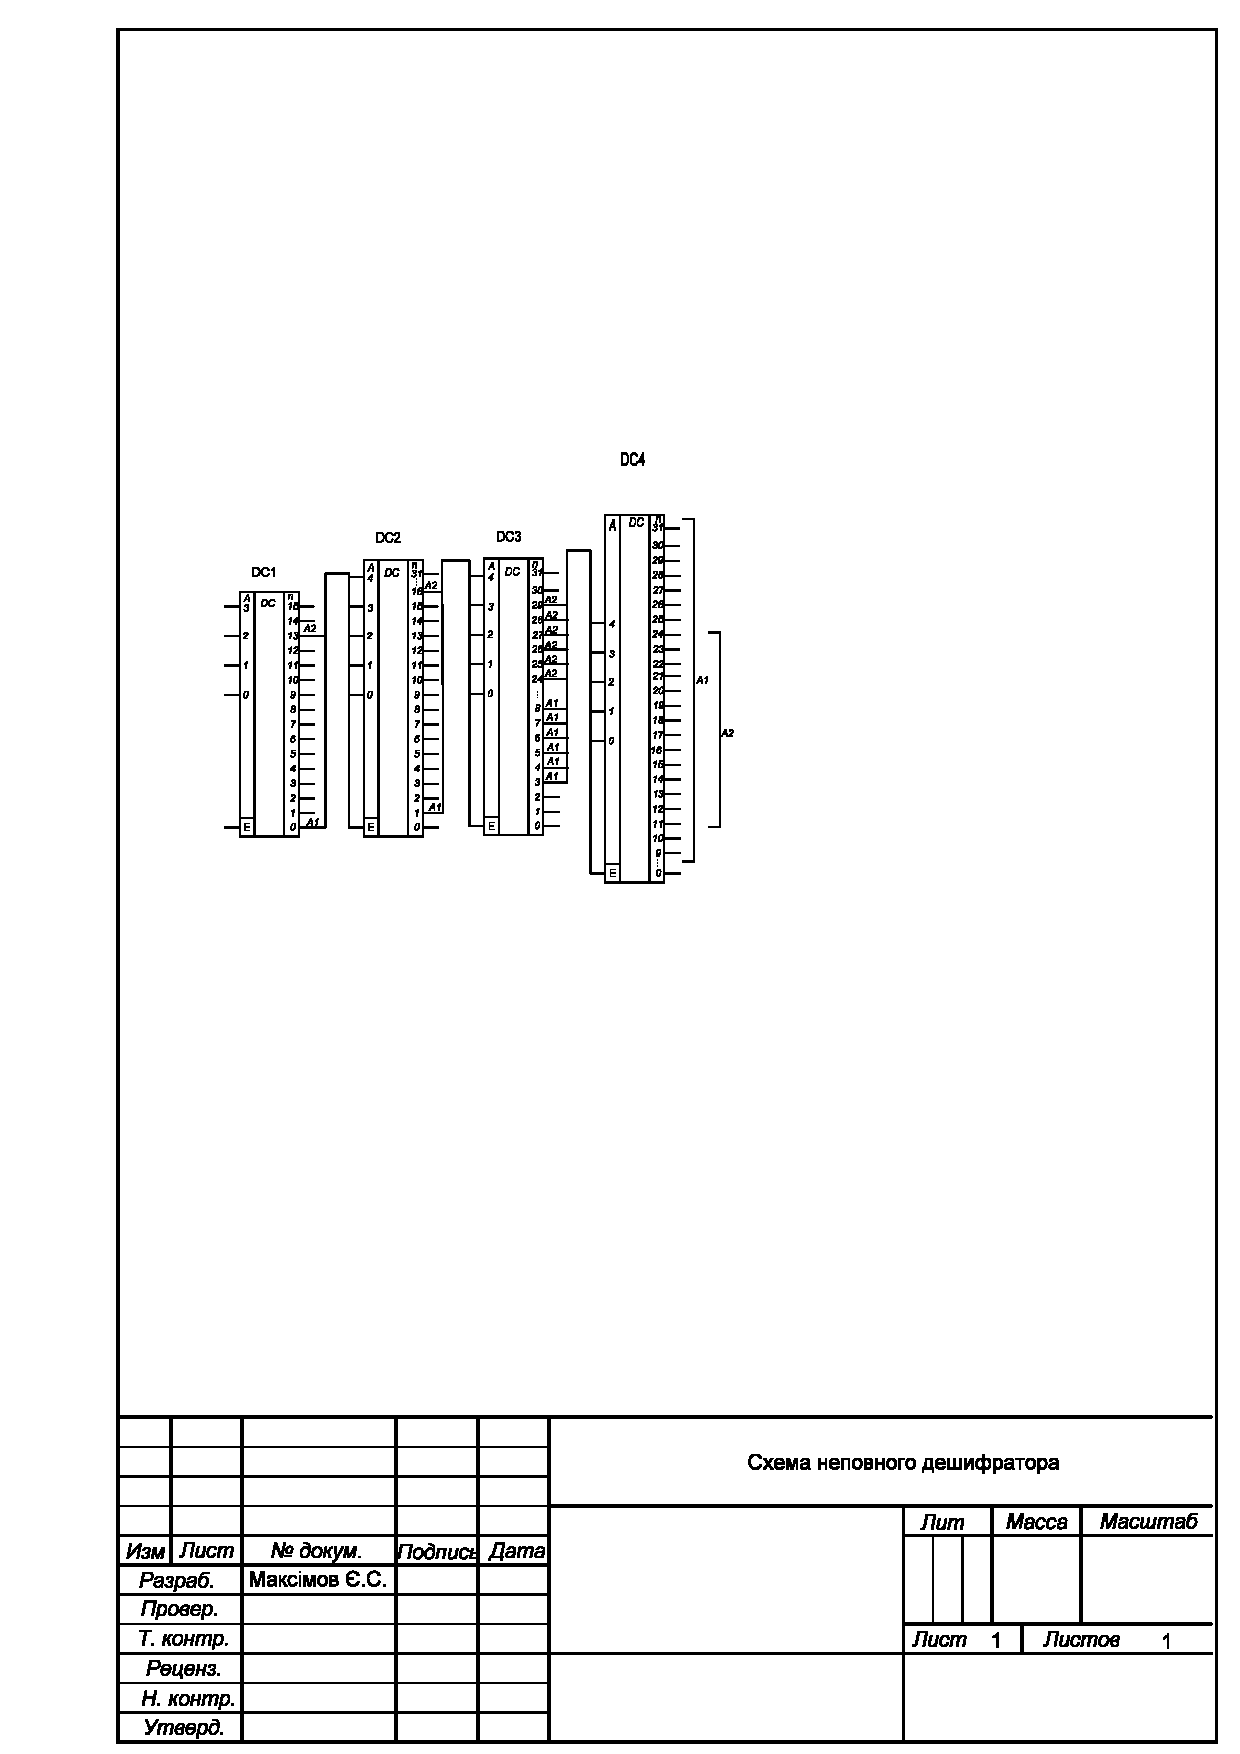
\includepdf[pages=-]{scheme_2.pdf}
\section{Апаратні витрати на побудову дешифратора}

\newpage
\chapter{Висновок}
